\pagestyle{fancy}
\rhead{\thepage}
\lhead{Introduction}
\chapter{Introduction}
% Add some introduction on sequencer

With the rapid development of digital audio technology, computers are playing an increasingly important role in music, and providing unprecedented opportunities for people to create and manipulate sound. The iPad, as portable computers with touch screen, offer musicians a new platform to express themselves. As a result, thousands of new musicial interfaces built on iPad have been created and played by musicians around the world. It is natural to ask, what kinds of musical interfaces design help musicians express themselves best? To answer this question, a new community called NIME emergeed from the establised field of human computer interaction(HCI) \citep{Reference16}. And in NIME, the evaluation of musical interface is mainly focused on expressivity, control and aethetic three aspects \citep{Reference0}. In this thesis, we are going to find out the common design patterns of music sequencer on iPad and trying to identify the strength and weakness of those interface design though a HCI user study.

% Talk anout creativity, control and aethetics....
\section{Background}
\label{sec: backgound}

\subsection{Development of Music Sequencer}
\label{subsec: history}
By modern definition, a music sequencer (or sequencer) is a hardware device or a software application which can handle several different forms of music materials such as notes and samples of sounds. It is widely used in performing electronic music, and used as a music processing tool in modern music composition. The history of music sequencer can refer to 9th century, the earlier sequencers worked as sound producing devices and depended on the preset inputs. A famous example of early stage music sequencer is player piano, a self-playing piano which play the music pre-recorded on a piano roll. When the technology matured, more forms of sequencer emerged. Analog sequencer which took advantage of analog eletronics was the first sequencer designed for live performance in addition to music composition. Step sequencer, also known as drum machine, distriputed the note into steps with equal time-interval, which free musicians from acurately timing of each note.

In morden times, digital sequencer implemented on computers become popular. The advent of Musical Instrument Digital Interface (MIDI) made the digital sequencer with great vitality. In recent years, the popularity of mobile devices brought music sequencers to a new platform and many new elements have been put into practice.

\subsection{iPad: a new playground for musicians}
\label{subsec: iPad}
% we will first brefly introduce the ipad, and then illustrate the strength of ipad. also the reason why we major investigate on ipad

The iPad, a portable computer with multi-touch screen, has quickly occupied the market all around world since it's first release in 2010 \citep{Reference2}. The emergence of iPad has provided a new platform for users to explore digital world \citep{Reference1}. After seven generations, the usage of iPad has shifted from a simple extension of iPhone to a powerful pruductivity tool. In this shift, thousands of applications which was designed to utilise the larger touch screen has emerged. According to \citeauthor{lifewire}, there are over 1.5 million apps currently hosted in the App Store, and more than half of those apps are specifically designed for iPad \citep{lifewire}.

Since the first release of iPad, there were practices to utilise the large tangible screen and wide variety of sensors on this cross-time product. \citeauthor{Reference8.4} designed \textit{Magic Fiddle}, a new musical instrument, which combined the physical gesture of users and graphical display of iPad together \citep{Reference8.4}. \citeauthor{Reference19} explored the possibility of using iPad as a percussive instrument and utilized iPad's network feature to ecourage cohesive improvisation among different users \citep{Reference19}.

\section{Related Work}

A lot of work have been down on evluating the interaction between users and mobile devices such as iPhone. However, there have not been a paper specificly analyze musical instrument implemented on mobile devices like iPad.

Although music sequencers were counted as the third most popular musical instrument apps on App Store \citep{Reference14}, we can barely find papers describe it's recent years development. The most related work was \textit{Block Jam} (see figure \ref{fig: Block Jam}), a sequencer with tangible interface consisited of several physical blocks \citep{Reference20}.

\bigskip
\begin{figure}[h]
  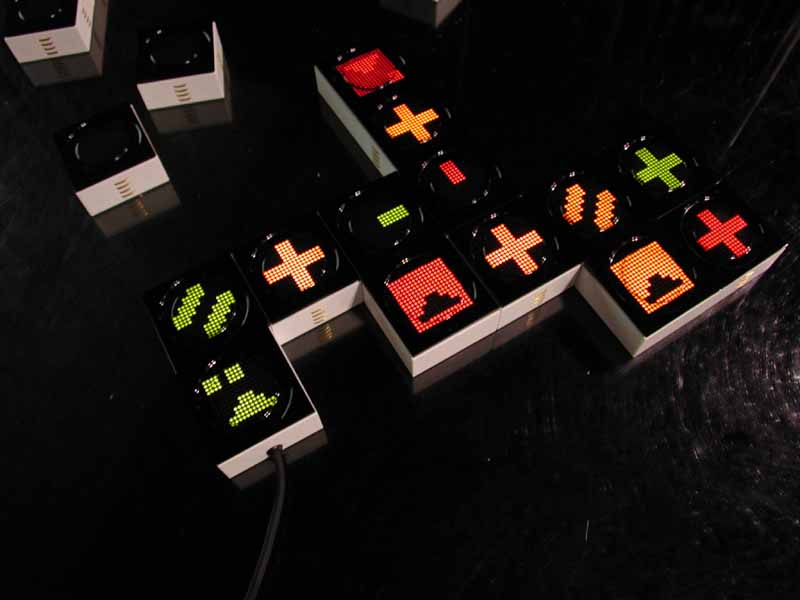
\includegraphics[width=12 cm]{images/blockjam.jpg}
  \centering
  \caption{Block Jam: music sequencer consist of a cluster of blocks}
  \label{fig: Block Jam}
\end{figure}
\bigskip

\section{Research motivation and goals}

While musical interfaces have been studied for a long time, there have emerged thousands of novel twists on \textquotedblleft{grid-based}\textquotedblright music sequencer. And to our knowledge there is currently no paper investigate the situation of this certain kind of musical application on App Store. What's more, there is no consensus on using what's method to evaluate those newborn musical application on mobile devices. This work is a first attempt to classify the music sequencers on iPad and adopt the evaluation method(MPX-Q Questionnaire) designed for NIME community. The goal of this thesis is to evaluate touch-based music sequencer apps on iPad by:
\begin{flushleft}
$\bullet$ Creating an interface taxonomy of current music sequencer apps on the iOS app store.\\
$\bullet$ Performing a HCI user study to measure user experience and musicians performance with different interface design approaches.\\
$\bullet$ Proposing design guidlines for musicians, developers and researcher for creating musical interface in the future.
\end{flushleft}

\section{Thesis structure}

In the next chapter, literature relevant to the research topic was introduced, so as to establish a theoretical framework of the research (see Chapter \ref{ch: chapter 2}). And the research project was divided into two consecutive studies. In the first study, we analyzed the music sequencer applications (designed for iPad) on App Store and create an interface taxonomy (see Chapter \ref{ch: chapter 3}). Then base on the classification of music sequencer interfaces, we selected one most representative application from each category and conducted an user study to evlauate the effect of different interface designs (see Chapter \ref{ch: chapter 4}). In Chapter \ref{ch: chapter 5}, we made a conclusion of the study and pointed out the future work.
